\documentclass{article}
\usepackage{graphicx}
\usepackage[utf8]{inputenc}
\usepackage[czech]{babel}
\usepackage{pdfpages}
\usepackage[margin=2.5cm]{geometry}
\usepackage{longtable,booktabs,array}
\usepackage{standalone}
\usepackage{enumitem}
\setlist[itemize]{label=-}
\usepackage{amsmath}
\usepackage{array}
\usepackage{tabularx}
\usepackage{hyperref}

\newcommand{\nt}[1]{\ensuremath{\langle\text{#1}\rangle}}
\newcommand{\term}[1]{\texttt{#1}}
\newcommand{\eps}{\ensuremath{\varepsilon}}
\newcommand{\ra}{\ensuremath{\rightarrow}}

% Don't include subsubsections in table of contents
\setcounter{tocdepth}{2} 

\title{\textbf{Implementace překladače \\
       imperativního jazyka IFJ26}}

\date{\today}

\begin{document}

    \maketitle
    \thispagestyle{empty}

    \subsection*{Autorský tým}
        \begin{tabular}{l l l l}
            \textbf{Roman Skoupý} & 281698 & \verb|xskoupr00| & autorský podíl 25 \%\\
            Matouš Jahoda & 281744 & \verb|xjahodm00| & autorský podíl 25 \%\\
            Tomáš Peňás & 281746 & \verb|xpenast00| & autorský podíl 25 \%\\
            Simon Šmíd & 282246 & \verb|xsmidsi00| & autorský podíl 25 \%\\
        \end{tabular}
        
    \subsection*{Zvolená varianta zadání}
        Tabulka s rozptýlenými položkami s implicitním zřetězením položek (TRP-izp)
        
    \subsection*{Implementovaná rozšíření}
        \begin{itemize}
            \item FUNEXP
            \item BOOLTHEN
            \item CONTROL
            \item VALMEM
            \item ALGEBDT
            \item LAMBDAS
            \item LISTS
            \item EXTKW
            \item PARAMLISTS
        \end{itemize}
        
    \subsection*{Git repozitář se zdrojovými kódy k projektu}
        \url{https://github.com/pes50/ifj}
        

    \newpage

    
    \tableofcontents
    \thispagestyle{empty}
    

    \newpage
    
    \section{Spolupráce}
        \subsection{Rozdělení práce}
            \begin{description}
                \item[Roman Skoupý] Vedení týmu, správa repozitáře, makefile, sémantický analyzátor, \\
                převod na vnitřní kód, testy, revize kódu
                \item[Matouš Jahoda] Syntaktický analyzátor, testy na syntaktický analyzátor, revize kódu
                \item[Tomáš Peňás] Tabulka symbolů, převod na vnitřní kód, generování cílového kódu, \\
                testy na tabulku symbolů, revize kódu, dokumentace
                \item[Simon Šmíd] Lexikální analyzátor, vyjádření vestavěných (builtin) funkcí ve vnitřním kódu, revize kódu
            \end{description}
            
        \subsection{Způsob spolupráce}
            Na úvodní schůzce jsme si rozdělili jednotlivé komponenty a následně každý pracoval na své části. Potřebná komunikace během práce na projektu probíhala hlavně zprávami přes Discord nebo přes audio hovory na\,Discordu. Pokud se problém netýkal celého týmu, domluva často probíhala také osobně.

            Některé komponenty nebyly na začátku přiděleny, a tak jsme je ve finální fázi projektu dělali společně, často přes hovor na Discordu a pomocí rozšíření Visual Studio Code \textit{Live share}.
            
            \subsubsection{Revize kódu}
                Na úvodní schůzce jsme se rozdělili do dvojic, které si navzájem měly dělat revizi kódu a potvrzovat žádosti o~začlenění do hlavní větve repozitáře. Nakonec ale revizi prováděl ten člen týmu, který měl v dané chvíli čas. V případech, kdy jsme na části kódu pracovali společně, vzájemně jsme svou práci kontrolovali již během psaní kódu a po dokončení jen jeden z autorů žádost vytvořil a druhý potvrdil.
            \subsubsection{Testování}
                Používali jsme jednotkové (kde jednotky jsou jednotlivé moduly překladače) i~integrační black-box testy. Až na několik málo výjimek byly testy vygenerovány s použitím umělé inteligence. Testy jsme vytvářeli až po\,implementaci jednotek (nevyužívali jsme metodiku \textit{Test-Driven Development}).
            \subsubsection{Formátování kódu}
                Využívali jsme formátovací styl \textit{LLVM} v nástroji \textit{ClangFormat} a pojmenovávací konvenci \textit{snake\_case}.
                
    \newpage
    

    \section{Architektura překladače}
        
            \begin{figure}[h]
                \centering
                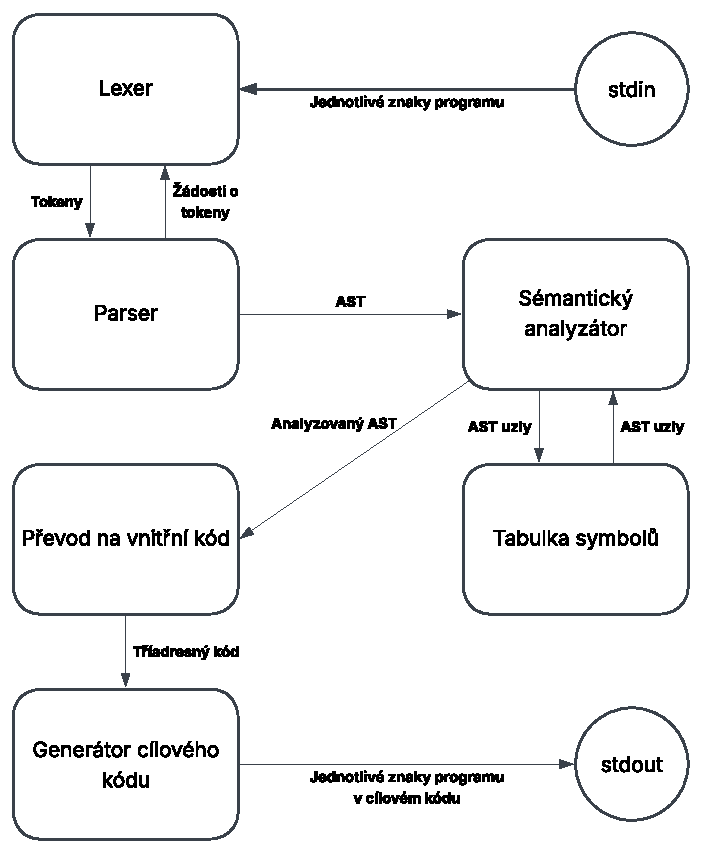
\includegraphics[scale = 1.2]{blokove_schema_ifj.pdf}
                \label{Blokové schéma překladače}
            \end{figure}
    
    
    \newpage


    \section{Popis jednotlivých modulů}
        \subsection{Lexikální analyzátor (Lexer)}
        Lexikální analyátor je sestaven ze souborů \verb|dynstr.c/.h|, \verb|expression_stack.c/.h|, \verb|indent_stack.c/.h|, a \verb|lexer.c/.h|. Převádí znaky ze vstupního proudu na tokeny a odsazení řeší pomocí zásobníku. Při rozpoznávání lexémů zohledňuje kontext předchozích tokenů a pro náhled tokenů dopředu využívá kruhový buffer.
            
            \subsubsection*{Konečný automat}
                Fungování lexeru v našem projektu je popsáno těmito automaty:
            
                \begin{figure}[h]
                    \centering
                    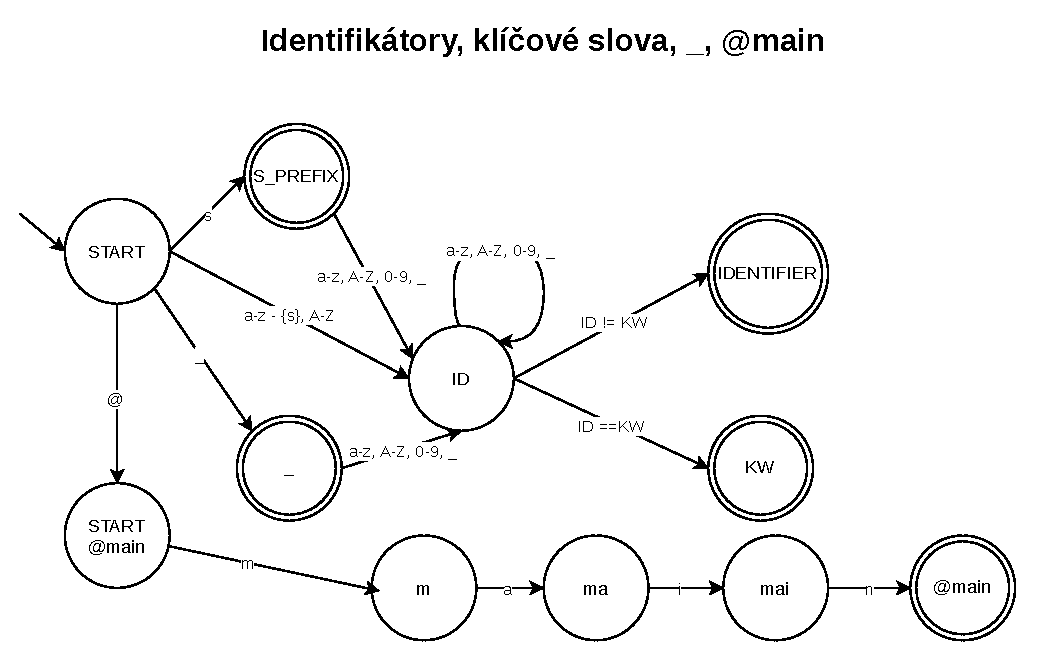
\includegraphics[scale = 1]{KA-lexer-1.pdf}
                    \label{Konečný automat pro identifikátory}
                \end{figure}

                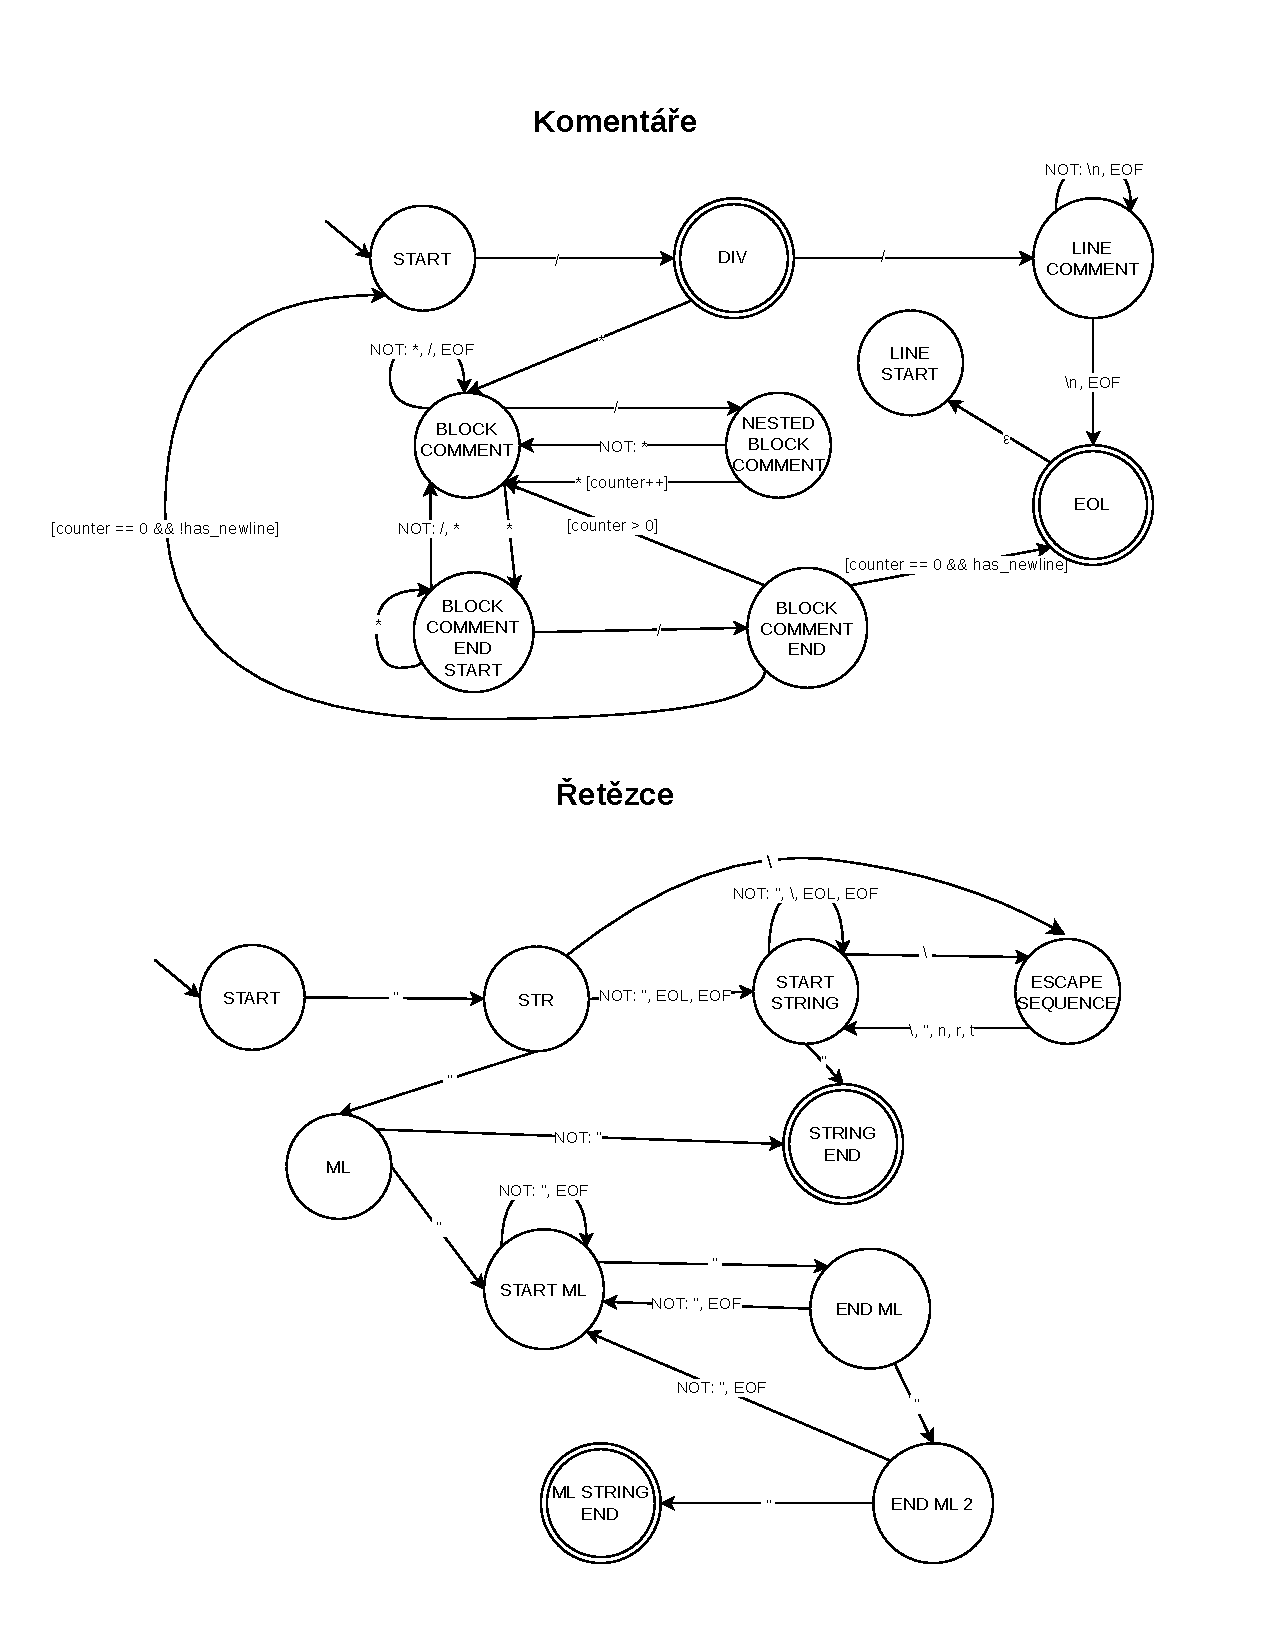
\includepdf[pages=-, pagecommand={\thispagestyle{plain}}]{KA-lexer-2.pdf}


        \newpage



        \subsection{Syntaktický analyzátor (Parser)}
            Parser obsahuje soubory \verb|parser.c/.h|, \verb|actions.c/.h|, \verb|token_stack.c/.h|. Hlavní část parseru využívá metodu rekurzivního sestupu a během syntaktické analýzy sestavuje celkový abstraktní syntaktický strom (AST) pomocí rozhraní z \verb|ast_node.h| a \verb|data_type.h|. Zpracování výrazů je řešeno samostatně pomocí precedenční tabulky a zásobníku, který uchovává tokeny a buduje dílčí podstrom daného výrazu.
            \subsubsection{LL gramatika}
                \input{ll_gramar}

            \subsubsection{LL tabulka}
                \input{ll_table}
            
            \subsubsection{Precedenční tabulka}
                \input{precedence_table}

        \subsection{Sémantický analyzátor}
            Sémantický analyzátor tvoří soubory \verb|analyse_block.c/.h|, \verb|analyse_callable_declarations.c/.h|,\\
            \verb|analyse_expression.c/.h|, \verb|analyse_types.c/.h|, \verb|semantic_analyser.c/.h|, \verb|builtin.c/.h|,\\
            \verb|collect_symbols.c/.h|, \verb|data_type.c/.h|,
            \verb|string_concatenate_dollar.c/.h| a \verb|string_duplicate.c/.h|. Sémantický analyzátor prochází AST dvakrát. Během prvního průchodu naplní tabulku symbolů, v druhém průchodu zkontroluje všechny deklarované funkce a typy. Pokud při analýze narazí na symbol, který ještě nebyl analyzován, přednostně ho zanalyzuje a teprve potom pokračuje v probíhající analýze.
        \subsection{Tabulka symbolů}
            Tabulka symbolů se skládá jen z dvojice souborů \verb|symtable.c/.h|. Jako tabulku symbolů jsme používali vázaný seznam (pseudo-zásobník, kde bylo možné přistupovat i k hlouběji uloženým prvkům) hašovacích tabulek, kde každá tabulka reprezentovala rozsah platnosti proměnné. Tabulka symbolů nevlastní žádná data symbolů, ale jen si ukládá ukazatel na příslušný uzel deklarace symbolu v AST. Pro rozptylování položek jsme využili Fowler–Noll–Vo hašovací algoritmus, konkrétně jeho variantu FNV-1a \cite{FNV-1a} s konstantami pro 32bitové hašování. Jako klíč jsme používali identifikátory symbolů. Kolize řeší tabulka lineárním sondováním s krokem velkým 1 prvek.
        \subsection{Převod na vnitřní kód}
            Převod na vnitřní kód se skládá ze souborů \verb|ast_convert.c/.h|, \verb|builtin_code.c/.h|,\\
            \verb|convert_expression.c/.h|, \verb|convert_list.c/.h|, \verb|convert_match.c/.h|, \verb|convert_node.c/.h|,\\ 
            \verb|convert_statements.c/.h|, \verb|inner_code.c/.h| a pomocné funkce má ve zvláštním souboru\\
            \verb|convert_utils.c/.h|. 
            Vnitřní kód je koncipován identicky s cílovým kódem (tříadresný kód se stejnými instrukcemi). Tato komponenta převádí konstrukce z AST na jednotlivé instrukce vnitřního kódu a ukládá je jako vázaný seznam, který předává generátoru kódu.
            
        \subsection{Generátor cílového kódu}
            Generátor cílového kódu obsahuje jen dvojici souborů \verb|codegen.c/.h|. Jelikož vnitřní kód byl navržen tak, aby~přesně odpovídal cílovému kódu, tato komponenta jen tiskne prvky vnitřního kódu na standardní výstup. 
            


    \newpage


    \section{Využití AI}
        Na úvodní schůzce týmu jsme se domluvili, že umělou inteligenci budeme používat výhradně pro testování a\,revizi kódu a tuto domluvu jsme dodrželi. Používali jsme modely Claude Sonnet 5.5, Gemini 3.1 Pro  a~Gemini Hydrogen. Umělou inteligenci jsme používali jen jako chatbota, nikoliv v agentním módu.

        Při generování testů jsme obvykle danému jazykovému modelu specifikovali, který soubor a jak má testovat. Chatbot dostal hlavičkový soubor a výpis pomocných funkcí s jejich argumenty. Dále jsme specifikovali, jak si má vytvořit pomocné struktury, či jak má vypadat správný výstup. Nakonec jsme vygenerovaný soubor zkontrolovali a upravili nebo přidali testované případy.
        
        Postup u revize probíhal různě v závislosti na velikosti revidovaných změn a také časových možnostech revidujícího člena týmu. 
        
        U změn menšího rozsahu jsme revizi prováděli manuálně a umělou inteligenci jsme nepoužívali. 
        
        Při revizi velkých změn, které bylo nutné zakomponovat do hlavní větve co nejdříve (například aby další člen týmu je mohl využívat v práci na své komponentě), jsme nejprve zkontrolovali práci s pamětí pomocí nástroje \textit{Valgrind} a\,následně nechali AI zkontrolovat krajní případy. Co se týče samotné funkcionality, spoléhali jsme hlavně na testy.  

        Během využívání AI jsme naráželi na problémy týkající se především velikosti kontextového okna. Zvláště s narůstající velikostí jednotlivých komponent bylo často nutné při revizi nechat model zpracovat požadavek několikrát, aby odhalil chyby, které při předchozím průchodu nenašel. Kvůli nedostatečné velikosti kontextového okna také často označoval některé části kódu za falešně chybné.

        
        

    \newpage

    
    \addcontentsline{toc}{section}{Převzaté zdroje}
    \def \refname {Převzaté zdroje}
    \begin{thebibliography}{99}
        \bibitem{FNV-1a} L. Noll, K. Vo, D. Eastlake 3rd, and T. Hansen, "The FNV Non-Cryptographic Hash Algorithm," RFC 9923, Feb. 2026. [Online]. Available: \mbox{\url{https://www.rfc-editor.org/info/rfc9923}}
    \end{thebibliography}
\end{document}
